\documentclass[../summary.tex]{subfiles}

\begin{document}
\section{Demography}
\subsection{Introduction}
\subsubsection{Population growth}

The global population has experienced a remarkable and rapid increase in recent history, but this growth has raised concerns about the Earth's capacity to sustain such numbers. Looking at the historical trajectory, we see that for most of human existence (approximately 300,000 years), the population remained relatively low, with just tens of millions of people on the planet. However, in the last 200 years, there has been an unprecedented surge, bringing the global population to around 8 billion.

\begin{figure}[H]
	\centering
	\begin{subfigure}{.5\textwidth}
		\centering
		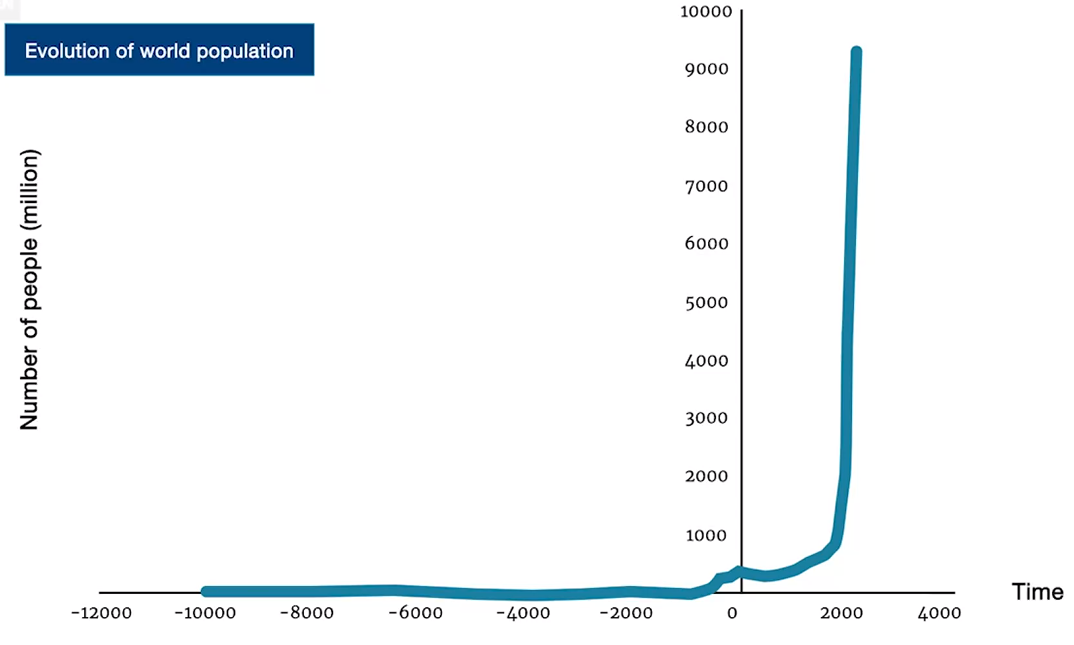
\includegraphics[width=1\linewidth]{../images/evolution_of_population}
		\caption{}
		\label{fig:evoltionofpopulation2}
	\end{subfigure}%
	\begin{subfigure}{.5\textwidth}
		\centering
		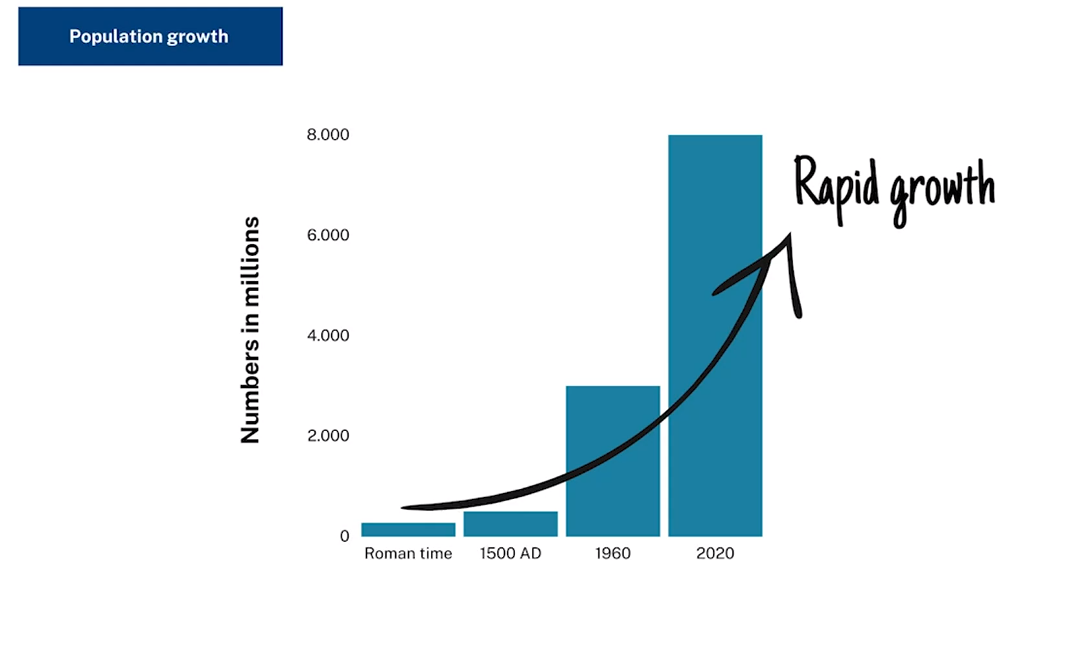
\includegraphics[width=0.9\linewidth]{../images/evolution_of_population_2}
		\caption{}
		\label{fig:evoltionofpopulation3}
	\end{subfigure}
	\caption{Evolution of the world population}
	\label{fig:evoltionofpopulation}
\end{figure}

\ \\
This rapid growth is a cause for concern for many, as some fear that it may lead to unsustainable pressure on the planet's resources and potential societal collapse. Reverend Thomas Malthus in the late 18th century and Paul Erlich in the 1960s both predicted such scenarios based on population growth.\\
\\
However, simply extrapolating from the past isn't sufficient to predict the future accurately. To gain a deeper understanding and insight, we must examine the mechanisms responsible for this recent population surge. We need to determine whether these mechanisms will continue to drive rapid population growth or if there are factors that may slow it down. By understanding these mechanisms, we can make informed projections and consider potential interventions to manage and control population growth.\\
\\
In essence, addressing the issue of population growth requires a scientific approach. We must delve into the historical and current factors driving population growth and use this knowledge to make more informed predictions about the future. This approach allows us to explore questions about the world's population in the coming decades and consider strategies to manage and reduce growth if deemed necessary.
\newpage

\subsection{History of mortality}
\subsubsection{Exponential growth}

Exponential growth is a fundamental concept often used to explain pessimistic views regarding population growth. It can be likened to the compound interest calculation used by banks, where a fraction of the existing capital is added each year. This results in a growing fraction being added as the total increases, leading to a rapidly accelerating growth curve.\\
 \\
Exponential growth is not confined to banking; it is observed in various aspects of life, including the spread of diseases like COVID-19, where the number of cases can grow exponentially. The key properties of exponential growth are its potential to reach any number, as there's no fixed limit, and acceleration over time.\\
\\
Critics of population growth point to this concept to express concerns about the Earth's capacity to sustain an ever-growing population. For instance, they argue that if each family has a certain number of children, and this pattern continues from one generation to the next, it would result in exponential population growth. However, this simplistic view doesn't account for the complexities of real-world demographics and population dynamics.\\
\\
To examine the issue, we should analyse population trends on a global scale over longer time periods, which can reveal whether growth is truly exponential or even more rapid, referred to as "super-exponential growth" .  On figure \ref{fig:evolutionoftheglobalpopulation}, the population is on a logarithmic axis. The population evolution does not plot as a straight line, but as a curve that is bending upwards. This means that the global population is growing even faster than exponential growth predicts. 
 
 \begin{figure}[H]
 	\centering
 	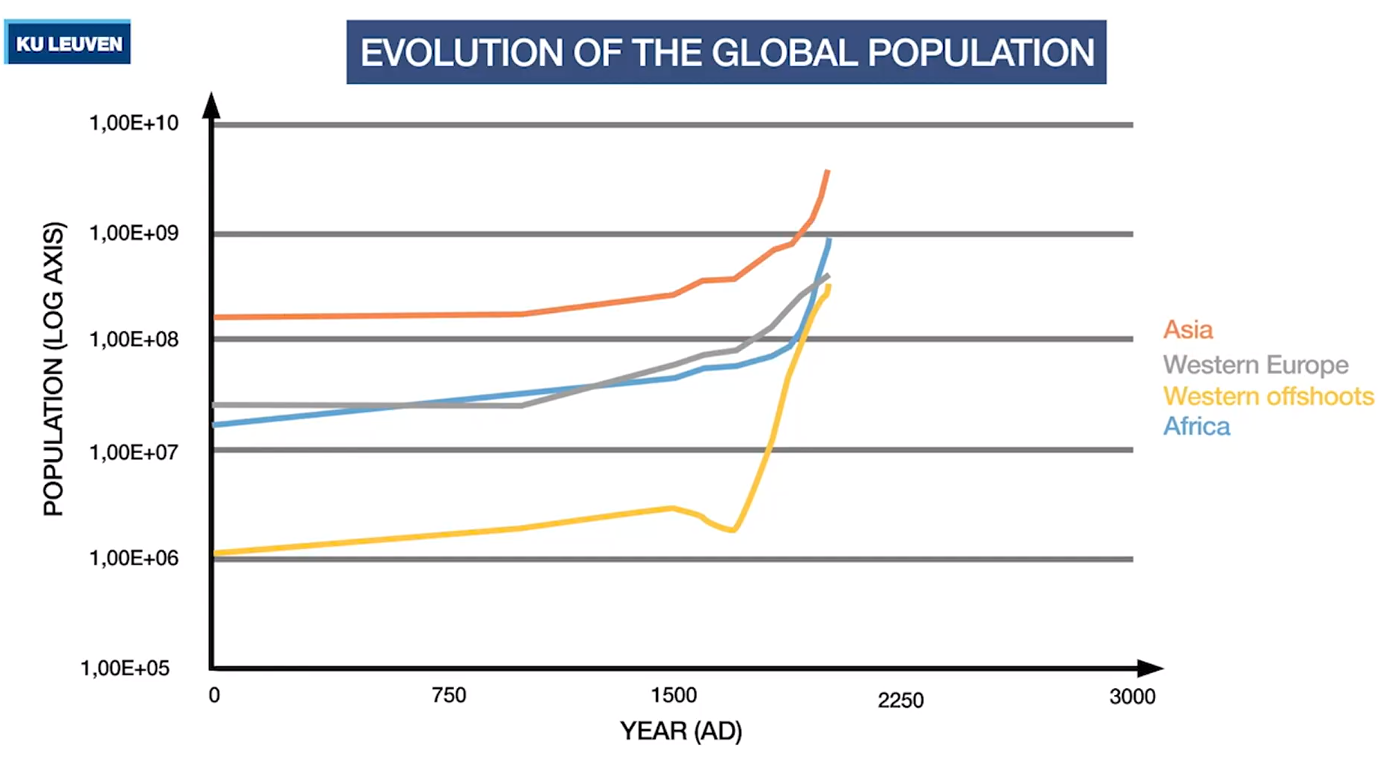
\includegraphics[width=0.8\linewidth]{../images/evolution_of_the_global_population}
 	\caption{Evolution of the global population}
 	\label{fig:evolutionoftheglobalpopulation}
 \end{figure}
 
 \ \\
 The latter is often seen as a potential crisis, as it can strain the capacity of systems to support the growing population. This leads to questions about whether the Earth can sustain such rapid growth, and if we can simply extrapolate past trends into the future.\\
 \\
 If we were to assume a 1\% annual growth rate, the Earth's population could exceed 20 billion people by the year 2122. This raises concerns about the planet's ability to support such a population. However, it's essential to consider whether this exponential growth will indeed persist, or if other factors and mechanisms will come into play to slow down population growth. This question remains a topic of ongoing research and debate.

\subsubsection{Industrial revolution}

The Industrial Revolution, which began in the 18th century, brought about significant changes in society and had a profound impact on health and mortality rates. Contrary to common perception, the introduction of industrialization led to a remarkable decline in mortality rates.\\
\\
Mortality rates in England, as well as in other countries experiencing the Industrial Revolution, started to decline from the very beginning of this transformation. Over a span of approximately 150 years, \textbf{mortality rates} in Great Britain were \textbf{halved}. This trend was not limited to one region; similar patterns emerged in countries undergoing industrialization.\\
\\
The key driver behind this decline in mortality was the increase in the availability of energy. The Industrial Revolution enabled society to extract more energy from the environment, which, in turn, transformed the mode of production and led to significant societal development.\\
\\
The availability of energy played a pivotal role in driving this transformation. To illustrate the magnitude of change, a single person working in a mine for a year could produce as much energy as is contained in a small jerrycan of diesel. That jerrycan represents just a fraction of the energy required to fuel a car. The vast increase in available energy fundamentally altered society.

\begin{figure}[H]
	\centering
	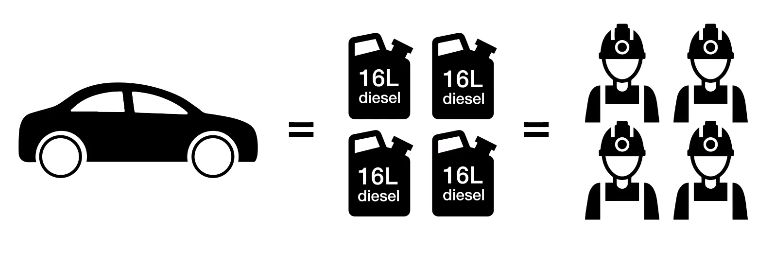
\includegraphics[width=0.7\linewidth]{../images/mine_worker}
	\caption{Energy comparison}
	\label{fig:mineworker}
\end{figure}
\ \\
The mode of production shifted from a predominantly rural setting where people worked on farms to an industrial society characterized by factories and machinery powered by fossil fuels. Workers in factories were initially inexperienced and required training. Factory owners who invested in training their workforce realized higher productivity and safety. Over time, those who provided training outperformed competitors who did not.\\
\\
Education and training provided not only the skills necessary for employment but also additional skills that improved individuals' abilities to reflect, discuss, understand their health, follow medical treatments, express their needs, and plan families. This marked a significant shift in society's capabilities.\\
\\
As industrialization progressed, society reorganized itself. Cities grew in importance, religion played a reduced role, and unions formed as workers could now collectively negotiate with factory owners. The demand for knowledge and technological advancement to improve efficiency in factories led to the development of science and technology. These advancements were not confined to industry but also extended to areas like healthcare, food production, and administrative efficiency (figure \ref{fig:reorganisationsociety}).

\begin{figure}[H]
	\centering
	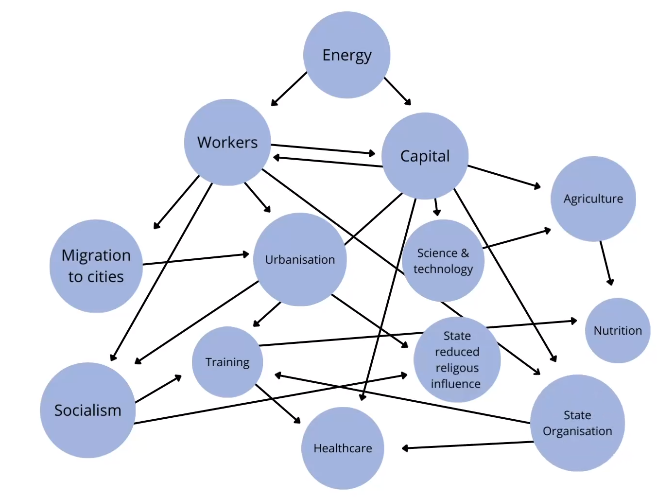
\includegraphics[width=0.7\linewidth]{../images/reorganisation_society}
	\caption{Reorganisation of the society since the industrialization}
	\label{fig:reorganisationsociety}
\end{figure}
\ \\
This combination of increased knowledge, societal organization, and technological advancements contributed to a dramatic reduction in mortality rates. The Industrial Revolution was not a detriment to health but, in fact, a driver of increased life expectancy and overall well-being.

\end{document}